\section{Graphentheorie}
\label{sec:graphentheorie}

Da GraphQL es ermöglicht, dass komplexe Beziehungen innerhalb eines Datenmodells in Form von Graphen modelliert werden~\cite[vgl. Modelling with Graph(QL)]{graphqlgraphtheory}
benötigt man die Graphentheorie, da diese Methoden liefert, um Graphen zu definieren und zu analysieren.
Des Weiteren sind die Testabdeckungskriterien, die später genutzt werden, eng mit der Graphentheorie verbunden.
Die folgenden Absätze werden eher theoretisch gehalten.
Die Zusammenhänge zwischen der Graphentheorie und Testen von GraphQL-APIs werden sich jedoch später erschließen.

\subsection{Ungerichteter Graph}

Ein Graph ist ein mathematisches Modell.
Es kann dazu verwendet werden, Beziehungen zwischen Objekten darzustellen.
Nach~\cite{graphentheorie} ist ein ungerichteter Graph wie folgt definiert:

\begin{definition}
    Ein ungerichteter Graph ist ein Paar $\textrm{G = (V, E)}$ zweier disjunkter Mengen mit E $\subseteq$ V^2
    \label{graphdef}
\end{definition}\cite[vgl. S.2 0.1 Graphen]{graphentheorie}
\\
\\
Die Elemente der Menge $V$ heißen Knoten (Vertices).
Verbindungen zwischen den Knoten sind Elemente der Menge $E$ und diese nennt man Kanten (Edges).
In dieser Definition spielt die Ordnung der Elemente von E keine Rolle, daher nennt man solche Graphen auch ungerichtete Graphen.
Um Graphen darzustellen, gibt es verschiedene Ansätze.
Der geläufigste Ansatz ist es, Knoten als Punkte und Kanten als Verbindungslinien zu zeichnen.
Häufig wird auch eine Adjazenzmatrix genutzt, bei dieser wird mit $0,1$ aufgeschlüsselt, welche Knoten eine Verbindung haben.
Bei $0$ existiert keine Kante zwischen den Knoten und bei $1$ existiert eine.

\begin{example}
    Ein Graph sei definiert mit $V = \{ 1, 2, 3 \}$ und $E = \{(1,1), (1,2), (1,3) \}$ \\
    Mögliche Darstellungen des Graphen sind in Abbildung~\ref{zeichnung} und~\ref{adjam} gezeigt.
    \label{exmgr}
\end{example}
    \begin{figure}[h!]
        \centering
        % Linke Seite: Code
        \begin{minipage}{0.45\textwidth}
            \centering
            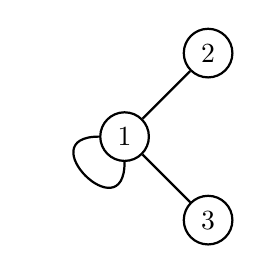
\begin{tikzpicture}[node distance={15mm}, thick, main/.style = {draw, circle}]
                \node[main] (1) {$1$};
                \node[main] (2) [above right of=1] {$2$};
                \node[main] (3) [below right of=1] {$3$};
                \draw (1) to [out=180,in=270,looseness=5] (1);
                \draw (1) -- (2);
                \draw (1) -- (3);
            \end{tikzpicture}
            \caption{Gezeichneter Graph}
            \label{zeichnung}
        \end{minipage}
        \hfill
        \begin{minipage}{0.45\textwidth}
            \centering
            \begin{array}{c|ccc}
                & 1 & 2 & 3 \\
                \hline
                1 & 1 & 1 & 1 \\
                2 & 0 & 0 & 0 \\
                3 & 0 & 0 & 0 \\
            \end{array}
            \caption{Adjazenzmatrix}
            \label{adjam}
        \end{minipage}
    \end{figure}

\subsection{Gerichteter Graph}

Gerichtete Graphen sind die Grundlage vieler Überdeckungskriterien~\cite[vgl. 2.1 Overview]{software-testing}.
Daher werden sie hier definiert.

\begin{definition}
    Ein gerichteter Graph ist ein Paar $\textrm{G = (V, E)}$ zweier disjunkter Mengen mit zwei Funktionen
    init: E \textrightarrow V und ter: E \textrightarrow V, die jeder Kante e eine Anfangsecke init(e) und eine
    Endecke ter(e) zuordnen~\cite[S.26 0.10 Verwandte Begriffsbildungen]{graphentheorie}.
    \label{gerichtetergraphdef}
\end{definition}

Bei einem gerichteten Graphen ist die Sortierung der Kantenpaare wichtig.
Die Funktionen $init$ und $ter$ können am einfachsten durch die Sortierung der Elemente eines Kantenpaares umgesetzt werden.
Hierbei ist das erste Element des Kantenpaares die Anfangsecke und das zweite Element ist die Endecke.
Die Kanten in einem gerichteten Graphen werden mit einem Pfeil gezeichnet.
Dabei zeigt der Pfeil stets in Richtung Endecke.
Der in Beispiel~\ref{exmgr} definierte ungerichtete Graph wird in Beispiel~\ref{exmggr} als gerichteter Graph angepasst.

\begin{example}
    \label{exmggr}
    Ein Graph sei definiert mit $V = \{ 1, 2, 3 \}$ und $E = \{e1, e2, e3\}$ \\
    Die Funktionen $init$ und $ter$ sind definiert als: \\
    $init(e1) = 1$ und $ter(e1) = 1$ \\
    $init(e2) = 1$ und $ter(e2) = 2$ \\
    $init(e3) = 1$ und $ter(e3) = 3$ \\
\end{example}

Nutzt man die Sortierung der Kanten für $init$ und $ter$, so sind $e1 = (1,1)$, $e2 = (1,2)$ und $e3 = (1,3)$.

\begin{figure}[H]
    \begin{center}
        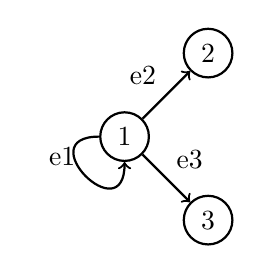
\begin{tikzpicture}[node distance={15mm}, thick, main/.style = {draw, circle}]
            \node[main] (1) {$1$};
            \node[main] (2) [above right of=1] {$2$};
            \node[main] (3) [below right of=1] {$3$};
            \draw[->] (1) to [out=180,in=270,looseness=5] node[midway, above left] {e1} (1);
            \draw[->] (1) -- node[midway, above left] {e2} (2);
            \draw[->] (1) -- node[midway, above right] {e3} (3);
        \end{tikzpicture}
    \end{center}
    \caption{ein gerichteter Graph}
    \label{graphexample}
\end{figure}

\subsection{Gewichteter Graph}

Für die spätere Entwicklung des Testentwurfs ist es wichtig, gewichtete Graphen zu definieren.
Zuvor wurde eine Kante in Definition~\ref{graphdef} und Definition~\ref{gerichtetergraphdef} als ein Tupel $(x, y)$ eingeführt.
Ein gewichteter Graph weist jeder Kante ein Kantengewicht zu.
Dies ist im Allgemeinen eine positive, reelle Zahl~\cite[vgl. S. 251]{graphentheorie3}.
Das Kantengewicht kann sowohl ungerichteten als auch gerichteten Kanten zugewiesen werden.

\begin{definition}
    Ein gerichteter/ungerichteter Graph G = (V,E) mit einer Abbildung g : E \textrightarrow $\mathbb{R}_{>0}$ heißt gerichteter/ungerichteter gewichteter Graph.
    Die Abbildung g heißt Gewichtsfunktion. Für $e \in E$ heißt g(e) das Gewicht von e.
    Das Gewicht von G ist die Summer der Gewichte aller Kanten, g(G) = \sum_{e \in G} g(e).\\
    \cite[vgl.~Definition~6.1~S.~251]{graphentheorie3}
    \label{gewichtetergraph}
\end{definition}
\\
\\
Für spätere Anwendungszwecke muss die Definition jedoch ein wenig allgemeiner gefasst werden.
Die Felder eines GraphQL-Typens sollen später als Gewicht genutzt werden um Tests zu entwerfen.
Um dies zu erleichtern, soll die Definition~\ref{gewichtetergraph} verallgemeinert werden durch eine Anpassung der Gewichtsfunktion.
Die neue Definition soll vorerst \textit{allgemein gewichteter Graph} genannt werden.

\begin{definition}
    Ein Graph G = (V,E) mit einer Abbildung g: E \textrightarrow X heißt allgemein gewichteter Graph.
    Die Menge X ist frei wählbar.
    \label{allgemeingewichtetergraph}
\end{definition}
An dieser Stelle sei verwiesen an Kapitel~\ref{testentwurf} wo diese Definition genutzt wird,
um Felder eines  GraphQL-Schemas den Kanten eines Graphens zuzuordnen.

\subsection{Pfad}
\label{pfad}

Ein Pfad, oft auch Weg genannt, ist eine Sequenz von Knoten, die nachfolgend durch Kanten miteinander verbunden sind~\cite[vgl. S. 7 0.3]{graphentheorie}.

\begin{definition}
    Ein Weg ist ein nicht leerer Graph P = (V,E) der Form $V = \{x_{0}, x_{1}, ..., x_{k}\}$ und $E = \{x_{0}x_{1}, x_{1}x_{2}, \ldots, x_{k-1}x_{k}\}$ wobei die $x_{i}$
    paarweise verschieden sind~\cite[vgl. S. 7]{graphentheorie}.
\end{definition}

Ein Weg wird oft durch die Folge seiner Knoten beschrieben also $P=x_{0} x_{1} \ldots x_{k}$ \cite[vgl. S.7]{graphentheorie}
Die Länge eines Weges ist die Anzahl der Kanten die dieser besucht~\cite[vgl. S. 7]{graphentheorie}.
In gewichteten Graphen ist das Gewicht eines Pfads die Summe aller Gewichte der einbezogenen Kanten~\cite[vgl. 7.2 kürzeste Wege]{graphentheorie3}.

\begin{example}
    Es sei ein gerichteter Graph G definiert mit V = $\{n1,n2,n3,n4,n5,n6,n7,n8\}$ und E = $\{(n1,n2),(n2,n3),(n3,n4),(n4,n1),(n2,n5),(n3,n6),(n5,n7),(n6,n8)\}$.
    Die Sortierung der Elemente von $E$ ist fest.
    Es gilt, dass $init(x)$ das erste Element des Kantenpaares ist.
    $ter(x)$ ist das zweite Element des Kantenpaares.
    Ein möglicher Pfad von Knoten $n1$ zu $n8$ ist der Pfad $p = \{(n1, n2), (n2, n3), (n3, n6), (n6, n8)\}$.
    Der Pfad p ist in Abbildung~\ref{pfadbsp} rot markiert \\ \\
\end{example}

\begin{figure}[H]
    \begin{center}
        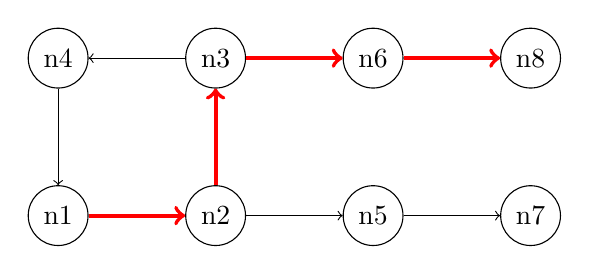
\begin{tikzpicture}
            \node[circle, draw] (n1) at (0,0) {n1};
            \node[circle, draw] (n2) at (2,0) {n2};
            \node[circle, draw] (n3) at (2,2) {n3};
            \node[circle, draw] (n4) at (0,2) {n4};
            \node[circle, draw] (n5) at (4,0) {n5};
            \node[circle, draw] (n6) at (4,2) {n6};
            \node[circle, draw] (n7) at (6,0) {n7};
            \node[circle, draw] (n8) at (6,2) {n8};

            \draw[->, red, line width=1.5pt] (n1) -- (n2);
            \draw[->, red, line width=1.5pt] (n2) -- (n3);
            \draw[->] (n3) -- (n4);
            \draw[->] (n4) -- (n1);
            \draw[->] (n2) -- (n5);
            \draw[->, red, line width=1.5pt] (n3) -- (n6);
            \draw[->] (n5) -- (n7);
            \draw[->, red, line width=1.5pt] (n6) -- (n8);
        \end{tikzpicture}
    \end{center}
    \caption{Pfad von n1 zu n8}
    \label{pfadbsp}
\end{figure}

\subsection{Kreis}

Ein Kreis in einem Graphen ist ein Weg, bei dem gilt: $Anfangsknoten = Endknoten$ \cite[vgl. S. 8]{graphentheorie}
Die Größe eines Kreises ist die Länge des Wegs, den dieser Kreis bildet.
Der kürzeste Kreis eines Graphens nennt sich $Taillenweite~g(G)$ und der längste Kreis ist der Umfang~\cite[vgl. S.8]{graphentheorie}.
Der Graph aus Beispiel~\ref{pfadbsp} hat einen Kreis der Länge 4 und ist in Abbildung~\ref{zyklgraph} rot eingezeichnet.

\begin{figure}[h!]
    \centering
    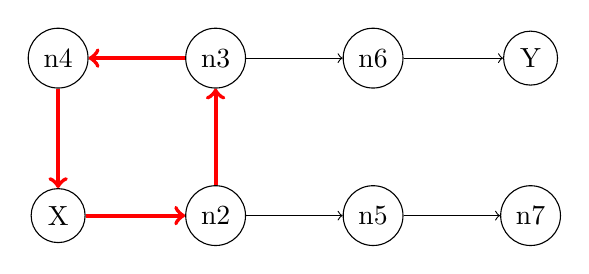
\begin{tikzpicture}
        \node[circle, draw] (n1) at (0,0) {X};
        \node[circle, draw] (n2) at (2,0) {n2};
        \node[circle, draw] (n3) at (2,2) {n3};
        \node[circle, draw] (n4) at (0,2) {n4};
        \node[circle, draw] (n5) at (4,0) {n5};
        \node[circle, draw] (n6) at (4,2) {n6};
        \node[circle, draw] (n7) at (6,0) {n7};
        \node[circle, draw] (n8) at (6,2) {Y};

        \draw[->, red, line width=1.5pt] (n1) -- (n2);
        \draw[->, red, line width=1.5pt] (n2) -- (n3);
        \draw[->, red, line width=1.5pt] (n3) -- (n4);
        \draw[->, red, line width=1.5pt] (n4) -- (n1);
        \draw[->] (n2) -- (n5);
        \draw[->] (n3) -- (n6);
        \draw[->] (n5) -- (n7);
        \draw[->] (n6) -- (n8);
    \end{tikzpicture}
    \caption{Ein zyklischer Graph}
    \label{zyklgraph}
\end{figure}

Im Kontext des Testentwurfs sind Kreise besonders interessant, da diese für einen potenziell unendlich großen Testraum sorgen.
In einem azyklischen gerichteten Graphen, also einem gerichteten Graphen, der keinen Kreis besitzt, ist die Menge aller möglichen Pfade endlich.
Bei einem Graphen mit Zyklen ist die Menge aller möglichen Pfade unendlich.
Dies folgt aus der Tatsache, dass jeder Pfad, der den Kreis beinhaltet, diesen Kreis ein weiteres Mal ablaufen kann und somit stets ein neuer Pfad generiert wird.

\newpage